% THIS DOCUMENT IS TAILORED TO REQUIREMENTS FOR SCIENTIFIC COMPUTING.  IT SHOULDN'T
% BE USED FOR NON-SCIENTIFIC COMPUTING PROJECTS
\documentclass[12pt]{article}

\usepackage{amsmath, mathtools}
\usepackage{amsfonts}
\usepackage{amssymb}
\usepackage{graphicx}
\usepackage{colortbl}
\usepackage{xr}
\usepackage{hyperref}
\usepackage{longtable}
\usepackage{xfrac}
\usepackage{tabularx}
\usepackage{float}
\usepackage{siunitx}
\usepackage{booktabs}
\usepackage{caption}
\usepackage{pdflscape}
\usepackage{afterpage}


\usepackage[round]{natbib}

%\usepackage{refcheck}

\hypersetup{
    bookmarks=true,         % show bookmarks bar?
      colorlinks=true,       % false: boxed links; true: colored links
    linkcolor=red,          % color of internal links (change box color with linkbordercolor)
    citecolor=green,        % color of links to bibliography
    filecolor=magenta,      % color of file links
    urlcolor=cyan           % color of external links
}

%% Comments

\usepackage{color}

\newif\ifcomments\commentstrue %displays comments
%\newif\ifcomments\commentsfalse %so that comments do not display

\ifcomments
\newcommand{\authornote}[3]{\textcolor{#1}{[#3 ---#2]}}
\newcommand{\todo}[1]{\textcolor{red}{[TODO: #1]}}
\else
\newcommand{\authornote}[3]{}
\newcommand{\todo}[1]{}
\fi

\newcommand{\wss}[1]{\authornote{blue}{SS}{#1}} 
\newcommand{\plt}[1]{\authornote{magenta}{TPLT}{#1}} %For explanation of the template
\newcommand{\an}[1]{\authornote{cyan}{Author}{#1}}

%% Common Parts

\newcommand{\progname}{ProgName} % PUT YOUR PROGRAM NAME HERE
\newcommand{\authname}{Team \#, Team Name
\\ Student 1 name
\\ Student 2 name
\\ Student 3 name
\\ Student 4 name} % AUTHOR NAMES                  

\usepackage{hyperref}
    \hypersetup{colorlinks=true, linkcolor=blue, citecolor=blue, filecolor=blue,
                urlcolor=blue, unicode=false}
    \urlstyle{same}
                                


% For easy change of table widths
\newcommand{\colZwidth}{1.0\textwidth}
\newcommand{\colAwidth}{0.13\textwidth}
\newcommand{\colBwidth}{0.82\textwidth}
\newcommand{\colCwidth}{0.1\textwidth}
\newcommand{\colDwidth}{0.05\textwidth}
\newcommand{\colEwidth}{0.8\textwidth}
\newcommand{\colFwidth}{0.17\textwidth}
\newcommand{\colGwidth}{0.5\textwidth}
\newcommand{\colHwidth}{0.28\textwidth}

% Used so that cross-references have a meaningful prefix
\newcounter{defnum} %Definition Number
\newcommand{\dthedefnum}{GD\thedefnum}
\newcommand{\dref}[1]{GD\ref{#1}}
\newcounter{datadefnum} %Datadefinition Number
\newcommand{\ddthedatadefnum}{DD\thedatadefnum}
\newcommand{\ddref}[1]{DD\ref{#1}}
\newcounter{theorynum} %Theory Number
\newcommand{\tthetheorynum}{TM\thetheorynum}
\newcommand{\tref}[1]{TM\ref{#1}}
\newcounter{tablenum} %Table Number
\newcommand{\tbthetablenum}{TB\thetablenum}
\newcommand{\tbref}[1]{TB\ref{#1}}
\newcounter{assumpnum} %Assumption Number
\newcommand{\atheassumpnum}{A\theassumpnum}
\newcommand{\aref}[1]{A\ref{#1}}
\newcounter{goalnum} %Goal Number
\newcommand{\gthegoalnum}{GS\thegoalnum}
\newcommand{\gsref}[1]{GS\ref{#1}}
\newcounter{stretchgoalnum} %Stretch Goal Number
\newcommand{\sgthestretchgoalnum}{STG\thestretchgoalnum}
\newcommand{\sgref}[1]{STG\ref{#1}}
\newcounter{instnum} %Instance Number
\newcommand{\itheinstnum}{IM\theinstnum}
\newcommand{\iref}[1]{IM\ref{#1}}
\newcounter{reqnum} %Requirement Number
\newcommand{\rthereqnum}{R\thereqnum}
\newcommand{\rref}[1]{R\ref{#1}}
\newcounter{nfrnum} %NFR Number
\newcommand{\rthenfrnum}{NFR\thenfrnum}
\newcommand{\nfrref}[1]{NFR\ref{#1}}
\newcounter{lcnum} %Likely change number
\newcommand{\lthelcnum}{LC\thelcnum}
\newcommand{\lcref}[1]{LC\ref{#1}}

\usepackage{fullpage}

\newcommand{\deftheory}[9][Not Applicable]
{
\newpage
\noindent \rule{\textwidth}{0.5mm}

\paragraph{RefName: } \textbf{#2} \phantomsection 
\label{#2}

\paragraph{Label:} #3

\noindent \rule{\textwidth}{0.5mm}

\paragraph{Equation:}

#4

\paragraph{Description:}

#5

\paragraph{Notes:}

#6

\paragraph{Source:}

#7

\paragraph{Ref.\ By:}

#8

\paragraph{Preconditions for \hyperref[#2]{#2}:}
\label{#2_precond}

#9

\paragraph{Derivation for \hyperref[#2]{#2}:}
\label{#2_deriv}

#1

\noindent \rule{\textwidth}{0.5mm}

}

\begin{document}

\title{Software Requirements Specification for \progname: RapidCare}
\author{\authname}
\date{\today}
	
\maketitle

~\newpage

\pagenumbering{roman}

\tableofcontents

~\newpage

\section*{Revision History}

\begin{tabularx}{\textwidth}{p{3cm}p{2cm}X}
\toprule {\bf Date} & {\bf Version} & {\bf Notes}\\
\midrule
Date 1 & 1.0 & Notes\\
Date 2 & 1.1 & Notes\\
\bottomrule
\end{tabularx}

\newpage

\pagenumbering{arabic}


\section{Introduction}

\subsection{Purpose of Document} \label{sec_PurposeOfDocument}

  The purpose of this document is to provide a comprehensive description of the requirements for a software application that aims to streamline the healthcare documentation process aimed to be run as a web application. This document will be used in as a contract in a sense between the team and the client who intends to use this application. This document will allow for an in-depth description of the software's functionality, performance, and other non-functional requirements. Additionally, it will outline common use-cases under which the software will be used. This will in turn provide a direction to the developers such that they will be empowered to creating the right product as this document will contain various stakeholders' requirements. Along with development direction, this document will be a direct reference for all of the stakeholders to understand the product's scope, functionality, and limitations.


\subsection{Characteristics of Intended Reader} \label{sec_IntendedReader} 

The intended readers of this SRS document include project managers, software developers, testing engineers, and stakeholders directly involved in the design and implementation of the software system. Project managers and testing engineers would be directly involved in the development and testing process. They would generally have an education in computer science along with experience in software design, web or mobile development, and software testing. Project managers generally have experience in managing software projects and knowledge of software development processes. Stakeholders like doctors and nursing staff would have domain knowledge and could provide insights to understand the clinical workflow and documentation process. 

\subsection{Scope of Requirements} \label{sec_ScopeOfRequirements}


\subsubsection{Context Overall Objective} \label{sec_ContextOverallObjective}

Ontario is facing an extreme shortage of family doctors, with the number of patients without one jumping by 600,000 to 2.5 million which is a growing number [1]. This situation is only to get worse as predicted by the Ontario Medical Association [2]. As a result, people find themselves going to the ER with coughs and colds and flooding the ER causing massive wait times which ends in patients even resulting in leaving without being seen [3]. A massive part of the wait time is due to the overhead of documentation tasks. Doctors, healthcare professionals, and support staff find themselves spending most of their time on documentation which overall slows the pipeline of patients tremendously.

\subsubsection{Expected Benefits} \label{sec_ExpectedBenefits}

The expected benefits of this project are as follows:
\begin{itemize}
  \item Reduced documentation overhead time
  \item Increased patient throughput
  \item Improved patient care
  \item Increased doctor and healthcare professional satisfaction
\end{itemize}

Much like how copilot is a tool for programmers, the aim is to create a tool for healthcare professionals to help with documentation such that the number of patient processed per day can be increased, and the focus of doctors and nurses can be shifted from documentation to patient care. 

\subsubsection{Goals} \label{sec_Goals}
The goals for this project are as follows:
\begin{table}[H]
    \centering
    \begin{tabular}{p{4cm} p{4cm} p{4cm}}
        \toprule
        \textbf{Goal} & \textbf{Definition} & \textbf{Rationale} \\
        \midrule
        G\refstepcounter{goalnum}\thegoalnum\label{G_VoiceToDocumentation}: Use voice to fill in medical documentation (charts, files, etc.) & The app will record conversations and automatically turn them into medical notes and charts. & This will save doctors time by automating paperwork, letting them focus more on patients. \\
        \midrule
        G\refstepcounter{goalnum}\thegoalnum \label{G_reduceOverhead}: Reduce documentation overhead time.  & Through tracking the whole patient journey in the app, we look to reduce the overhead of triaging, clinical documentation, and other registrations.  & This helps hospital healthcare professionals focus on care and lowers the time taken through registration for hospital staff. \\ 
        \midrule
        G\refstepcounter{goalnum}\thegoalnum \label{G_integrateEnv}: Integrates with the existing hospital environment. & We want the solution to be portable such that it can be implemented in existing hospital and clinic ecosystems.  & Portability will ensure that hospitals and clinics won’t have to upgrade their existing hardware to use the application. \\
        \midrule 
        G\refstepcounter{goalnum}\thegoalnum \label{G_hNetworkProfiles}: Allow health networks profiles with in service. & Need the ability for health networks to add, update, and delete network profile details. & This will ensure that the list of hospitals and staff in the network is up to date with appropriate permissions. \\
        \midrule 
        G\refstepcounter{goalnum}\thegoalnum \label{G_hProfessionalProfiles}: Allow health care professional profiles with in service. & Need the ability for health networks to add, update, and delete staff profile details. & This will ensure that the list of staff will be able to use the tool to dictate patient conversations or add other notes. Additionally, making sure they have access to patient journey. \\
        \midrule 

    \end{tabular}
\end{table}

\subsubsection{Stretch Goals} \label{sec_StretchGoals}
The stretch goals for this project are as follows:
\begin{table}[H]
    \centering
    \begin{tabular}{p{4cm} p{4cm} p{4cm}}
        \toprule
        \textbf{Goal} & \textbf{Definition} & \textbf{Rationale} \\
        \midrule
        STG\refstepcounter{stretchgoalnum}\thestretchgoalnum \label{STG_medicineSuggestions}: Automated medicine suggestions. & Based on diagnosis and patient data provide medicine suggestions. & This will help doctors fill out their charts faster. \\ % Row 1
        \midrule
        STG\refstepcounter{stretchgoalnum}\thestretchgoalnum \label{STG_diagnosisSuggestions}: Automated diagnosis suggestions.  & Use AI to suggest possible diagnoses based on what the doctor and patient discuss.  & This will help doctors make faster, more accurate diagnoses, especially in tricky cases.\\ 
        \midrule
        STG\refstepcounter{stretchgoalnum}\thestretchgoalnum \label{STG_triage}: Increase efficiency for triage.  & Create functionality to prioritize patients based on the severity of their condition. & This ensures the most critical patients get treated first, improving care in emergencies. \\
        \bottomrule
    \end{tabular}
\end{table}


\subsection{Organization of Document} \label{sec_OrganizationOfDocument}

The organization of this document is as follows:
\begin{itemize}
  \item \textbf{System Description}\\
  This section will provide an overview of the system, its functionality, the characteristics of the users, and the constraints of the system.
  \item \textbf{Requirements}\\
  This section will outline the functional and non-functional requirements. Additionally, it will provide a rationale for all of the requirements.
  \item \textbf{Likely Changes}\\
  This section will outline the likely changes that may occur in the future.
  \item \textbf{Unlikely Changes}\\
  This section will outline the unlikely changes that may occur in the future.
  \item \textbf{References}\\
  This section will provide a list of references used in the document.

\end{itemize}

~\newpage

\section{System Description} \label{sec_SystemDescription}

\subsection{Definitions, Acronyms, and Abbreviations} \label{sec_DefinitionsAcronymsAbbreviations}

\begin{tabular}{l l} 
  \toprule    
  \textbf{symbol} & \textbf{description}\\
  \midrule 
  A & Assumption\\
  G & Goals\\
  STG & Stretch Goals\\
  FR & Functional Requirement\\
  NFR & Non-functional Requirement\\
  LC & Likely Change\\
  ULC & Unlikely Change\\
  SRS & Software Requirements Specification\\
  EHR & Electronic Healthcare Record\\
  
  \bottomrule
\end{tabular}\\

The following is the glossary for this document:

\begin{itemize}
  \item \textbf{System:} When referring to a system the document refers to the intended solution/product.
  \item \textbf{User:} When referring to a user the document refers to a person who will use the product.
  \item \textbf{Healthcare Professional:} When referring to healthcare professionals the document refers to doctors, nurses, and other healthcare professionals who will be using the product.
  \item \textbf{Patient:} When referring to a patient the document refers to any person who is receiving medical treatment.
  \item \textbf{Healthcare Network:} When referring to a healthcare network the document refers to an organisation that has group of hospitals or clinics and will use the system.

\end{itemize}


\subsection{System overview} \label{sec_SystemOverview}

Through this project we aim to develop a solution that will address key niche problems through customizability and add features of critical need that do not already exist in existing solutions. This will allow healthcare networks to centralize the data of their hospitals and increase the staff productivity.\\

\noindent This product has been conceived by the group members based on elicitation. Through interviews and discussion the problem of documentation overhead was found. This is the problem to be solved for the capstone course SFWRENG 4G06.

\subsection{System Functionality} \label{sec_SystemFunctionality}

This section outlines the core functionalities and characteristics of the proposed system:

\begin{itemize}
  \item \textbf{Patient Documentation:} The system should facilitate efficient and streamlined patient documentation throughout the EHR documentation process. This includes storing patient data, clinical notes, treatment plans, and patient history in a secure manner.
  
  \item \textbf{Voice Transcription:} The system should be able to record conversations between healthcare professionals and patients which will be transcribed to fill out charts and patient profiles efficiently.
  
  \item \textbf{Real-time Data Access:} The users must have real-time access to patient data and documentation enabling them to make informed decisions quickly and efficiently.
  
  \item \textbf{Automated Medicine Suggestions:} The system should be able to provide automated medicine suggestions based on the transcribed data which will help users to fill out the charts faster and make informed treatment decisions.
  
  \item \textbf{Automated Diagnosis Suggestions:} The system should be able to suggest possible diagnoses based on transcribed data which will help users to make faster and more accurate diagnoses.
  
  \item \textbf{User Authentication:} The system must provide secure user authentication methods to ensure that only authorized personnel can access sensitive patient information.
  
\end{itemize}


\subsection{User Characteristics} \label{sec_UserCharacteristics}

The intended users of this product are healthcare professionals, specifically those involved in patient documentation, including doctors, nurses, and other clinical administrative staff. \\

The following are the user characteristics associated with the intended users:\\

\textbf{Education Level:} All users are expected to have a minimum of a college diploma and basic reading, writing, and speaking skills. The education level of the intended users will vary based on their role, generally a bachelor’s degree or college diploma in nursing, medicine, or other healthcare fields. \\

\textbf{Experience:} All users will be expected to have basic familiarity with EHR systems or similar applications. This experience will depend on their roles ranging from entry-level positions to experienced professionals. \\

\textbf{Technical Expertise:} The users should have basic technical skills to use EHR systems and other healthcare software applications. In addition to this, the users should have familiarity with data entry processes and analytics interpretation. \\

\textbf{Accessibility Considerations:} It is anticipated that some users may have accessibility issues. The user interface should be designed for ease of navigation, incorporating various accessibility features.\\

Specific requirements must be specified to accommodate users with varying technical expertise and diverse educational backgrounds. This will ensure the application is usable by all healthcare staff, regardless of their abilities.


\subsection{System Constraints}

The following constraints will guide the system design and implementation:

\begin{itemize} 

  \item \textbf{Compliance with Regulatory Standards:} The system must adhere to healthcare regulations ensuring the confidentiality and security of patient data.

  \item \textbf{User Accessibility:} The system must meet established accessibility standards to ensure usability for all healthcare staff, including those with disabilities.

  \item \textbf{Cost and Time:} The system must be developed within the imposed budget and time restrictions.

\end{itemize}

\subsubsection{Assumptions and Dependencies} \label{sec_assumpt}

\begin{itemize}
  \item\textbf{Reliable Internet Connection} -- We are assuming that user has a reliable internet connection throughout the patient’s visit as it is essential for authentication to the app, real-time interaction with it, running updates and saving the document to the patient’s profile.
  \item\textbf{Sufficient Hardware Accessories} -- We are assuming that the user has the required hardware devices such as monitors, iPads etc. to access the system.
  \item\textbf{Patient’s Consent} -- We also assume that medical staff will obtain patients’ consent when required.
\end{itemize}

\subsubsection{Usage Scanerios}

Here are the use-case scenarios for this software--

\begin{itemize}
  \item\textbf{UC1 Login} --
  \begin{itemize}
    \item The user accesses the system using an internet browser.
    \item The user enters valid credentials on the log in page.
    \item The user selects the login button.
    \item The user lands on the default dashboard.
  \end{itemize}
  \item\textbf{UC2 Recording Clinical Notes} --
  \begin{itemize}
    \item The user accesses patient’s record.
    \item The user selects dictate button.
    \item The user dictates the notes and hit the stop button.
    \item The user reviews the transcribed text.
    \item The user selects the submit button.
  \end{itemize}
  \item\textbf{UC3 Diagnostic Suggestions} --
  \begin{itemize}
    \item The user submits the transcribed text.
    \item The user reviews the potential diagnostic suggestions.
    \item The user accepts or rejects suggestions.
  \end{itemize}
  \item\textbf{UC4 Create Patient Profile} --
  \begin{itemize}
    \item The user log into the system.
    \item The user selects the ‘create a new record’ button.
    \item The user provide input for the required fields.    
    \item The user selects the submit button.
  \end{itemize}
\end{itemize}

\textbf{Usage Scenario 1 : Documenting a Patient Consultation}

\begin{itemize}
  \item\textbf{Use Case} -- UC2, UC3
  \item\textbf{Primary Actor} -- Healthcare professional (such as a medical doctor or a nurse)
  \item\textbf{Precondition} -- The user has been successfully authenticated, logged into the system and has patient’s profile is created. The basic information such as name, contact information, and history is prefilled.
  \item\textbf{Trigger} -- The user will press the dictate button.
  \item\textbf{Main Success Scenario} --
  \begin{itemize}
    \item The user will press the dictate button.
    \item The system will convert audio to text in real-time.
    \item The user will press stop button.
    \item The user reviews the transcribed notes. 
    \item The system has accurately transcribed the audio to text without any inaccuracies.
    \item The user selects the submit button after review. 
  \end{itemize}
  \item\textbf{Secondary Success Scenario} --
  \begin{itemize}[label=5.\arabic*]
    \item The system has produced some inaccuracies in the transcribed text.
    \begin{itemize}[label=5.1\arabic*]
      \item The user selects the edit button.
      \item The system prompts user to edit the text.
      \item The user manually edits the transcribed text.
    \end{itemize} 
  \end{itemize}
  \item\textbf{Success Postcondition} --
  \begin{itemize}
    \item The notes are successfully saved in patient database and changes are reflected in the user interface.
  \end{itemize}
\end{itemize}

\begin{figure}[h]
  \centering
  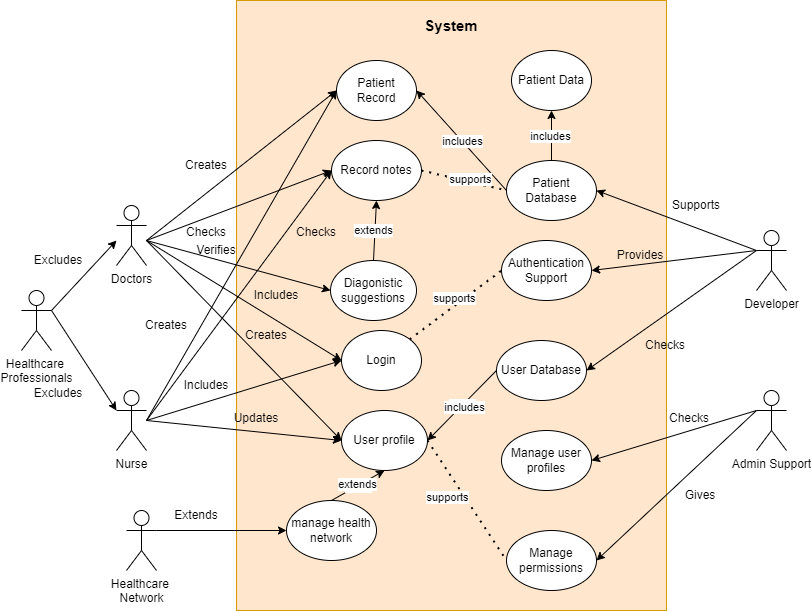
\includegraphics[width=0.8\textwidth]{use-case.drawio.png}
  \caption{This is the use-case diagram for this project.}
  \label{fig:Use-Case Diagram}
\end{figure}

\subsubsection{Risks and Mitigation}

Looking at implementation details there are a few risks that come up, if these risks can be addressed or have a clearer roadmap that will make us more confident in the project. 

\begin{itemize}
  \item \textbf{Speech Input} -- A hospital or a clinic can be a loud place, in the event audio input is taken we need to ensure that it is clean and clear. This would mean essentially blocking outside noise. 
  \item \textbf{Visual Inputs} -- If any old charts need to be inputted into the patient journey having the ability to scan and transfer the information into the required format will be another risk. The document needs to be rid of noisy data.
  \item \textbf{Pre-Trained Models} -- To manipulate and use both inputs above we need to create a model to be accurate and provide accuracy when filling in charts. 
  \item \textbf{Data Privacy} -- This application will hold a lot of patient data so creating a store that is secure and making sure standard data security practice is applied is a must.
  \item \textbf{User Acceptance} -- This will require further elicitation from outside supervisors. We need to gather data on what critical needs of healthcare professionals such that critical features are present.
  \item \textbf{Technical Delay} -– Integration with Electronic Health record systems might cause some delays if there’s any technical issue or if the software faces compatibility issues. This will require sample testing to make sure that the software is compatible in the early stage of the development process.
  \item \textbf{Professional Verification} -– Misinterpretation of some words might lead to inaccurate records and wrong diagnosis. Therefore, it’s important for the doctor/nurse to verify the final version of the document and manually delete anything that was falsely recorded. 
\end{itemize}

~\newpage

\section{Requirements} \label{sec_Requirements}


\subsection{Functional Requirements} \label{sec_FunctionalRequirements}


\noindent \begin{itemize}

\item[FR\refstepcounter{reqnum}\thereqnum \label{FR_meaningfulLabel}:] 

\textbf{Requirement:} Add healthcare network

\textbf{Fit Criterion:}  

\textbf{Dependencies:}  

\textbf{Monitored and Controlled Variables:} 

\textbf{Performance Requirements:} 

\textbf{Hardware Requirements:} 

\textbf{Software Requirements:} 

\textbf{Normal Behavior:} 

\textbf{Undesired Event Handling:} 


\item[FR\refstepcounter{reqnum}\thereqnum \label{FR_meaningfulLabel}:]  

\textbf{Requirement:} Remove healthcare network 

\textbf{Fit Criterion:}  

\textbf{Dependencies:}  

\textbf{Monitored and Controlled Variables:} 

\textbf{Performance Requirements:} 

\textbf{Hardware Requirements:} 

\textbf{Software Requirements:} 

\textbf{Normal Behavior:} 

\textbf{Undesired Event Handling:} 

\item[FR\refstepcounter{reqnum}\thereqnum \label{FR_meaningfulLabel}:] 

\textbf{Requirement:} Update healthcare network

\textbf{Fit Criterion:}  

\textbf{Dependencies:}  

\textbf{Monitored and Controlled Variables:} 

\textbf{Performance Requirements:} 

\textbf{Hardware Requirements:} 

\textbf{Software Requirements:} 

\textbf{Normal Behavior:} 

\textbf{Undesired Event Handling:} 

\item[FR\refstepcounter{reqnum}\thereqnum \label{FR_meaningfulLabel}:]

\textbf{Requirement:} Add healthcare professionals

\textbf{Fit Criterion:}  

\textbf{Dependencies:}  

\textbf{Monitored and Controlled Variables:} 

\textbf{Performance Requirements:} 

\textbf{Hardware Requirements:} 

\textbf{Software Requirements:} 

\textbf{Normal Behavior:} 

\textbf{Undesired Event Handling:} 

\item[FR\refstepcounter{reqnum}\thereqnum \label{FR_meaningfulLabel}:] 

\textbf{Requirement:} Remove healthcare professionals.

\textbf{Fit Criterion:}  

\textbf{Dependencies:}  

\textbf{Monitored and Controlled Variables:} 

\textbf{Performance Requirements:} 

\textbf{Hardware Requirements:} 

\textbf{Software Requirements:} 

\textbf{Normal Behavior:} 

\textbf{Undesired Event Handling:} 

\item[FR\refstepcounter{reqnum}\thereqnum \label{FR_meaningfulLabel}:] 

\textbf{Requirement:} Update the list of healthcare professionals. 

\textbf{Fit Criterion:}  

\textbf{Dependencies:}  

\textbf{Monitored and Controlled Variables:} 

\textbf{Performance Requirements:} 

\textbf{Hardware Requirements:} 

\textbf{Software Requirements:} 

\textbf{Normal Behavior:} 

\textbf{Undesired Event Handling:} 


\item[FR\refstepcounter{reqnum}\thereqnum \label{FR_meaningfulLabel}:] 

\textbf{Requirement:} Allow users to log in.

\textbf{Fit Criterion:}  

\textbf{Dependencies:}  

\textbf{Monitored and Controlled Variables:} 

\textbf{Performance Requirements:} 

\textbf{Hardware Requirements:} 

\textbf{Software Requirements:} 

\textbf{Normal Behavior:} 

\textbf{Undesired Event Handling:} 


\item[FR\refstepcounter{reqnum}\thereqnum \label{FR_meaningfulLabel}:] 

\textbf{Requirement:} create a patient record.

\textbf{Fit Criterion:}  

\textbf{Dependencies:}  

\textbf{Monitored and Controlled Variables:} 

\textbf{Performance Requirements:} 

\textbf{Hardware Requirements:} 

\textbf{Software Requirements:} 

\textbf{Normal Behavior:} 

\textbf{Undesired Event Handling:} 

\item[FR\refstepcounter{reqnum}\thereqnum \label{FR_meaningfulLabel}:] 

\textbf{Requirement:} Delete the patient record.

\textbf{Fit Criterion:}  

\textbf{Dependencies:}  

\textbf{Monitored and Controlled Variables:} 

\textbf{Performance Requirements:} 

\textbf{Hardware Requirements:} 

\textbf{Software Requirements:} 

\textbf{Normal Behavior:} 

\textbf{Undesired Event Handling:} 

\item[FR\refstepcounter{reqnum}\thereqnum \label{FR_meaningfulLabel}:] 

\textbf{Requirement:} Update the patient record by typing - allow the user to edit the transcribed data

\textbf{Fit Criterion:}  

\textbf{Dependencies:}  

\textbf{Monitored and Controlled Variables:} 

\textbf{Performance Requirements:} 

\textbf{Hardware Requirements:} 

\textbf{Software Requirements:} 

\textbf{Normal Behavior:} 

\textbf{Undesired Event Handling:} 

\item[FR\refstepcounter{reqnum}\thereqnum \label{FR_meaningfulLabel}:] 

\textbf{Requirement:} Update the patient record by dictation -ability to record. 

\textbf{Fit Criterion:}  

\textbf{Dependencies:}  

\textbf{Monitored and Controlled Variables:} 

\textbf{Performance Requirements:} 

\textbf{Hardware Requirements:} 

\textbf{Software Requirements:} 

\textbf{Normal Behavior:} 

\textbf{Undesired Event Handling:} 

\item[FR\refstepcounter{reqnum}\thereqnum \label{FR_meaningfulLabel}:] 

\textbf{Requirement:} transcribe conversation to text in real time. 

\textbf{Fit Criterion:}  

\textbf{Dependencies:}  

\textbf{Monitored and Controlled Variables:} 

\textbf{Performance Requirements:} 

\textbf{Hardware Requirements:} 

\textbf{Software Requirements:} 

\textbf{Normal Behavior:} 

\textbf{Undesired Event Handling:} 

\item[FR\refstepcounter{reqnum}\thereqnum \label{FR_meaningfulLabel}:] 

\textbf{Requirement:} provide diagnostic suggestions based on the transcribed data.

\textbf{Fit Criterion:}  

\textbf{Dependencies:}  

\textbf{Monitored and Controlled Variables:} 

\textbf{Performance Requirements:} 

\textbf{Hardware Requirements:} 

\textbf{Software Requirements:} 

\textbf{Normal Behavior:} 

\textbf{Undesired Event Handling:} 

\item[FR\refstepcounter{reqnum}\thereqnum \label{FR_meaningfulLabel}:] 

\textbf{Requirement:} provide a list of frequently used medicines based on diagnosis.

\textbf{Fit Criterion:}  

\textbf{Dependencies:}  

\textbf{Monitored and Controlled Variables:} 

\textbf{Performance Requirements:} 

\textbf{Hardware Requirements:} 

\textbf{Software Requirements:} 

\textbf{Normal Behavior:} 

\textbf{Undesired Event Handling:} 

\item[FR\refstepcounter{reqnum}\thereqnum \label{FR_meaningfulLabel}:] 

\textbf{Requirement:} send patient journey to another provider.

\textbf{Fit Criterion:}  

\textbf{Dependencies:}  

\textbf{Monitored and Controlled Variables:} 

\textbf{Performance Requirements:} 

\textbf{Hardware Requirements:} 

\textbf{Software Requirements:} 

\textbf{Normal Behavior:} 

\textbf{Undesired Event Handling:} 

\end{itemize}


\subsection{Non-functional Requirements} \label{sec_NonFunctionalRequirements}

\noindent \begin{itemize}

\item[NFR\refstepcounter{nfrnum}\thenfrnum \label{NFR_LookAndFeel}:] \textbf{Aesthetic and Design}

    \textbf{Requirement:} The UI should keep a clean design, that fits the healthcare standards.

    \textbf{Rationale:} A clean user interface allows users to navigate through the application with ease.

    \textbf{Fit Criterion:} UI demos will be sampled to healthcare workers to ensure that the design is easily understood and user-friendly.

    \textbf{Dependencies:} Design feedback loops and UX/UI design software.  

    \textbf{Undesired Event Handling:} If the surveys shows less than 80\% satisfaction, the design will then be revised.


\item[NFR\refstepcounter{nfrnum}\thenfrnum \label{NFR_Usability}:] \textbf{Usability}

    \textbf{Requirement:} The UI of the system should be intuitive, allowing healthcare workers to master its use with a training of up to 30 minutes. 

    \textbf{Rationale:} If the UI is user-friendly, it tends to reduce the learning time and allows health care workers to focus on patients.
  

    \textbf{Fit Criterion:} Tests that demonstrates that atleast 90\% of healthcare workers are able to navigate the system with 30 minutes of training or less.

    \textbf{Dependencies:} Feedback on the design during the development of the system.

    \textbf{Undesired Event Handling:} The system should support the user using a live chat support integrated within the application.

\item[NFR\refstepcounter{nfrnum}\thenfrnum \label{NFR_Performance}:] \textbf{Performance}

    \textbf{Requirement:} The system should convert voice recordings into text onto medical charts within 30 seconds of recording.

    \textbf{Rationale:} Reduces the documentation time to reduce workload and allow healthcare workers to focus on patients.
    
    \textbf{Fit Criterion:} The system will consistently generate completed documentation within 30 seconds of recording completion.  

    \textbf{Dependencies:} Speech-to-text engine.  

    \textbf{Undesired Event Handling:} The system will reduce any background processes, if it fails to generate completed documentation within 30 seconds.

\item[NFR\refstepcounter{nfrnum}\thenfrnum \label{NFR_Operational}:] \textbf{Operational Requirement}

    \textbf{Requirement:} The system should have an uptime guarantee of 99.9\% during operational hours.

    \textbf{Rationale:} Reliable uptime ensures consistent system for healthcare workers, specially in time-sensitive atmospheres like hospitals.

    \textbf{Fit Criterion:} System logs will confirm an uptime rate of 99.9\% over a 30-day period.  

    \textbf{Dependencies:} Cloud infrastructure and local hardware resilience. 
    
    \textbf{Undesired Event Handling:} There should be backup servers that turn on within 10 seconds of downtime to ensure reliable uptime.

\item[NFR\refstepcounter{nfrnum}\thenfrnum \label{NFR_Maintainability}:] \textbf{Maintainability Requirement}

    \textbf{Requirement:} The system should be updated with new features without causing downtime longer than 2 minutes.

    \textbf{Rationale:} Easily maintained system allows for consistent service.

    \textbf{Fit Criterion:} Release logs will show updates occur with less than 2 minutes of downtime.  

    \textbf{Dependencies:} Continuous integration of updates to the system.  

    \textbf{Undesired Event Handling:} If an update fails, the system will automatically revert to the last stable version.

\item[NFR\refstepcounter{nfrnum}\thenfrnum \label{NFR_Security}:] \textbf{Security Requirement}

    \textbf{Requirement:} The system should have all patient data encrypted, and in compliance with HIPAA standards.

    \textbf{Rationale:} A secure and confidential system ensures the user to be confident in using the application.

    \textbf{Fit Criterion:} Security audits will show 100\% compliance with HIPAA and encryption standards.  

    \textbf{Dependencies:} Encryption services and security protocols.  

    \textbf{Undesired Event Handling:} If a security breach is detected, all users will be logged out, access will be locked, and administrators alerted.

\item[NFR\refstepcounter{nfrnum}\thenfrnum \label{NFR_Cultural}:] \textbf{Cultural Requirement}

    \textbf{Requirement:} The system should allow customization of language settings to accommodate all healthcare workers.

    \textbf{Rationale:} A customized UI allows the user to feel comfortable and confident when using the application.

    \textbf{Fit Criterion:} Tests will show that healthcare workers can navigate through the application and switch languages based on their preference without impacting the functionality of the application.

    \textbf{Dependencies:} Language bundles.  

    \textbf{Undesired Event Handling:} If a language bundle fails to load, the system will revert to the default language and notify the user.

\item[NFR\refstepcounter{nfrnum}\thenfrnum \label{NFR_Legal}:] \textbf{Legal Requirement}

    \textbf{Requirement:} The system should comply with all healthcare data protection regulations. 

    \textbf{Rationale:} Legal compliance is mandatory to protect patient data and avoid penalties.  

    \textbf{Fit Criterion:} Legal audits will confirm compliance with HIPAA and any other relevant data protection laws.  

    \textbf{Dependencies:} Legal consultancy, data protection regulations.  

    \textbf{Undesired Event Handling:} If the system fails to comply with regulations, it will be updated within 24 hours to meet compliance.

\end{itemize}

\subsection{Rationale}

\plt{Provide a rationale for the decisions made in the documentation.  Rationale
should be provided for scope decisions, modelling decisions, assumptions and
typical values.}

\section{Likely Changes}    

\noindent \begin{itemize}

\item[LC\refstepcounter{lcnum}\thelcnum\label{LC_meaningfulLabel}:] \plt{Give
    the likely changes, with a reference to the related assumption (aref), as appropriate.}

\end{itemize}

\section{Unlikely Changes}    

\noindent \begin{itemize}

\item[ULC\refstepcounter{lcnum}\thelcnum\label{LC_meaningfulLabel}:] \plt{Give
    the unlikely changes.  The design can assume that the changes listed will
    not occur.}

\end{itemize}

~\newpage

\section{References}

\newpage{}
\section*{Appendix --- Reflection}

\wss{Not required for CAS 741}

The information in this section will be used to evaluate the team members on the
graduate attribute of Lifelong Learning.  

The purpose of reflection questions is to give you a chance to assess your own
learning and that of your group as a whole, and to find ways to improve in the
future. Reflection is an important part of the learning process.  Reflection is
also an essential component of a successful software development process.  

Reflections are most interesting and useful when they're honest, even if the
stories they tell are imperfect. You will be marked based on your depth of
thought and analysis, and not based on the content of the reflections
themselves. Thus, for full marks we encourage you to answer openly and honestly
and to avoid simply writing ``what you think the evaluator wants to hear.''

Please answer the following questions.  Some questions can be answered on the
team level, but where appropriate, each team member should write their own
response:


\begin{enumerate}
  \item What went well while writing this deliverable? 
  \item What pain points did you experience during this deliverable, and how did
  you resolve them?
  \item How many of your requirements were inspired by speaking to your
  client(s) or their proxies (e.g. your peers, stakeholders, potential users)?
  \item Which of the courses you have taken, or are currently taking, will help
  your team to be successful with your capstone project.
  \item What knowledge and skills will the team collectively need to acquire to
  successfully complete this capstone project?  Examples of possible knowledge
  to acquire include domain specific knowledge from the domain of your
  application, or software engineering knowledge, mechatronics knowledge or
  computer science knowledge.  Skills may be related to technology, or writing,
  or presentation, or team management, etc.  You should look to identify at
  least one item for each team member.
  \item For each of the knowledge areas and skills identified in the previous
  question, what are at least two approaches to acquiring the knowledge or
  mastering the skill?  Of the identified approaches, which will each team
  member pursue, and why did they make this choice?
\end{enumerate}

\end{document}